%%%%%%%%%% Beamerの初期設定 %%%%%%%%%%%
% beamerを使用する初期設定
\documentclass[aspectratio=169, 12pt, dvipdfmx]{beamer}

% パッケージ読み込み
% 下記のように color / xcolor を追加で読み込む場合は、ドライバオプションは付けずに
\usepackage{graphicx}
\usepackage{lmodern}
\usepackage{amsmath, amssymb, bm,hyperref}
\usepackage{physics}
\usepackage{cite}
\usepackage[version=4]{mhchem}
%デザインの選択 (省略可)
\usetheme{Default}
%%%%%%%%%%%%%%%%%%%%%%%%%%%%%%%%%%%%%


%%%%%%%%%% Beamerの基本的なコード %%%%%%%%%%
% 属性

\title{有限温度におけるSn核の超流動相転移解析\\Woods-Saxonポテンシャルと\\seniority pairingモデルの応用}
\author{根岸 颯}
\date{February 28, 2025} % あるいは特定の日付
\setbeamertemplate{footline}[frame number]
\begin{document}

\begin{frame}
  \titlepage
\end{frame}

\begin{frame}
  
\end{frame}


\begin{frame}{概要}
  原子核のenergy scaleは1MeV $\simeq 10^{10}$K程度であるため、
  地上においてこのような熱平衡状態が実現されるとは考えられず、
  通常扱う原子核はT=0Kにあるとみなしても問題は生じない。
  しかし、恒星内部やその終焉時等の極限環境下においての温度は10億K以上になるため、
  原子核は有限温度の熱浴の下にあると考えることができる。
  有限温度の原子核の性質は、核融合反応等への応用が期待される。
  ここでは、\ce{{}^{100-132}Sn}核を例に取り、Woods-Saxon potentialとseniority pairingモデルを用いた解析を試みる。
\end{frame}

\section{理論}

% \begin{frame}{Woods-Saxonポテンシャル}
%   有限井戸ポテンシャル、調和振動子ポテンシャルと比較し、より現実の原子核の性質を反映するポテンシャル。
%   原子核の密度分布と同じ形。
%   パラメータ$R,a$は、それぞれ、原子核の半径と表面のぼやけである。
% \end{frame}

\begin{frame}{Woods-Saxonポテンシャル}
  \begin{columns}[totalwidth=1.0\linewidth]
    \begin{column}[t]{0.45\linewidth}
      \begin{itemize}
        \item $V(r)=\dfrac{V_0(< 0)}{1+\exp((r-R)/a)}$
        \item より現実の原子核の性質を反映。
        \item 原子核の密度分布と同じ形。
        \item パラメータ$R,a$は、それぞれ、原子核の半径と表面のぼやけ。
      \end{itemize}
    \end{column}

    \begin{column}[T]{0.55\linewidth}
      \centering
      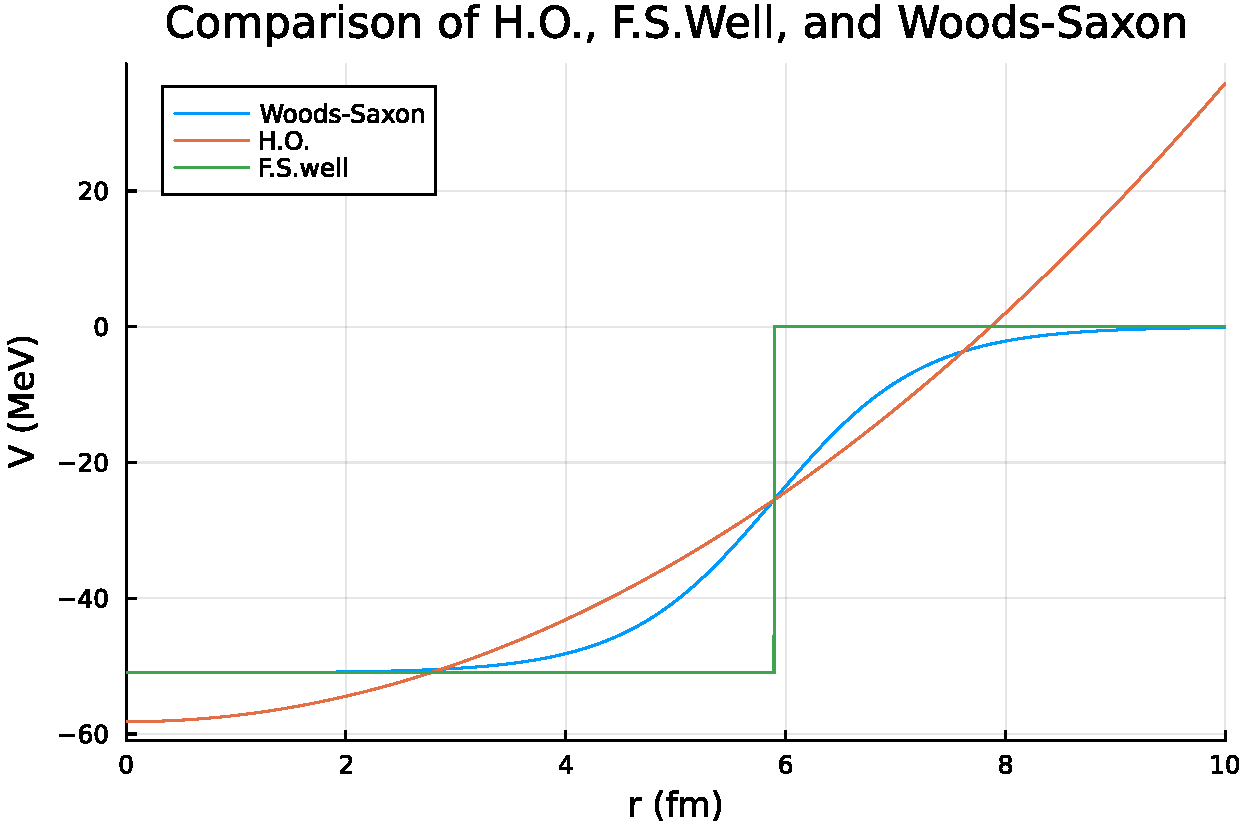
\includegraphics[width=\textwidth]{Comp_pt.pdf}
      \vspace{5pt} % キャプションと画像の間隔調整
      \scriptsize 図1:
  \end{column}
  \end{columns}
\end{frame}

\begin{frame}{平均場近似における単粒子Hamiltonian}
  Woods-Saxonポテンシャルを採用し、Hamiltonianを
  3次元極座標運動エネルギー$T_{\text{HO}}=\hbar\omega\left(2n+l+\frac{3}{2}\right)$
  を用いて
  \begin{equation}
    H=T_{\text{HO}}+U(r)
  \end{equation}
  と定義する。このときのポテンシャル$U(r)$は、
  \begin{equation}
    U(r)=u_0f(r)+u_{ls}r_0^2\dfrac{1}{r}\dfrac{df(r)}{dr}\boldsymbol{l}\cdot\boldsymbol{s}+U_{Coul}(r)\dfrac{1-\tau}{2}:f(r)=\dfrac{1}{1+\exp\left(\frac{r-R}{a}\right)}
  \end{equation}
  である。\\
  このHamiltonianを対角化することで単粒子エネルギーを求める。
\end{frame}

\begin{frame}{seniorityモデルにおけるHamiltonian}
  残留相互作用を含めた
  Hamiltonian  $H'$を数演算子$N_j$,quasi-spin 演算子$S_{j+}$を用いて
  \begin{equation}
    H' = \sum_j \epsilon_j N_j\ -\ gS_{+} S_{-}\quad;S_{+} \equiv \sum_j S_{j+}\ ,\ S_{-} \equiv (S_{+})^\dagger
  \end{equation}
  のように定める。このとき$j$は$N=50\sim 82$を満たす軌道である。
\end{frame}


%BCS理論の説明。どのような理論なのか、どうして原子核に適用できるのか。
%方程式自体は次のスライドで
\begin{frame}{BCS理論}
  引力に対する対相関力に対しては$J=0$対が多くの準位に分布し、分布の仕方が
  多数あるため、seniority数(未ペア粒子数)が低い状態で表されてしまい、独立な状態が多数存在する。
  これを説明する理論として超伝導を説明する理論であるBCS理論が採用される。
  \cite{asakura_structure}
  この分布のうち、最もエネルギーが低い基底状態を変分法的に求められ、この状態が"超伝導"状態となっている
  その基底状態はパラメータ$v_k,u_k$を用いて
  \begin{equation}
    \ket{\text{BCS}}=\prod_{k>0}\left(u_k + v_k a^{\dagger}_{k}a^{\dagger}_{\bar{k}}\right)\ket{0},
  \end{equation}
  と表される。
\end{frame}

\begin{frame}{BCS方程式}
  BCSパラメータ$v_k,u_k$は、単粒子エネルギー$\epsilon$,化学ポテンシャル$\lambda$,ギャップ$\Delta$を用いて、\cite{thenuclearmanybody}
  \begin{equation}
    \left. 
      \begin{aligned}
        u_k^2\\
        v_k^2
      \end{aligned}
    \right\}
    =\dfrac{1}{2}\left(1\pm\dfrac{\epsilon_k -\lambda}{\sqrt{(\epsilon_k -\lambda)^2+\Delta_k^2}}\right)
  \end{equation}
  と表される。またパラメータを決める方程式として粒子数方程式、ギャップ方程式が用いられ、
  \begin{align}
    \Delta  &=  g\sum_{k>0}u_k v_k\label{Gap T=0}\\
    N       &=  2\sum_{k>0}v_k^2\label{number T=0}
  \end{align}
\end{frame}

\begin{frame}{有限温度BCS理論}
  熱力学的分布に従うため、Fermi分布$f_i=1/(1+\exp(\beta E_i))$を用いて有限温度の場合に対して書き直すと、式(\ref{Gap T=0}),(\ref{number T=0})は
  \begin{align}
    \Delta  &=  g\sum_{k>0}u_k v_k(1-2f_i)\label{Gap FT}\\
    N       &=  2\sum_{k>0}\left[v_k^2+(u_k^2 - v_k^2)f_i\right]\label{number FT} 
  \end{align}
  のように書き直される。
\end{frame}

\begin{frame}{手順}
  \begin{enumerate}
    \item 単粒子エネルギーを求める。
    \item seniorityモデルを用いてpairing strength $g$を求める。
    \item 以上を用いて有限温度BCS計算を行い、相転移を追う。
  \end{enumerate}
\end{frame}

\section{計算手法}

\begin{frame}{計算に用いた方程式1}
  ポテンシャルパラメータ$u_{0},u_{ls}$はそれぞれ、
  \begin{align}
    r_0=1.27\ ,\ R=r_0A^{1/3}\ ,\ a=0.67\ [\text{fm}]\\
    u_0=\left(-51+33\dfrac{N-Z}{A}\right),u_{ls}=\left(22-14\dfrac{N-Z}{A} \right)\ [\text{MeV}]
  \end{align}
    以上を用いて波動関数$\psi_{nlj}$を基底に用いてハミルトニアンを構成し、対角化を行う。
\end{frame}

\begin{frame}{計算に用いた方程式2}
  gap$\Delta$は、偶奇質量差から求める。$\Delta=\dfrac{1}{2}(E_{g.s.}^{(N+1)}+E_{g.s.}^{(N-1)}-2E_{g.s.}^{(N)})$であり、
  基底エネルギーと結合エネルギーの関係として、$E_{g.s.}^{(N)}=-B(N)+Const.$を用いて
  計算する。ここで結合エネルギーは、
  \begin{equation}
    B(Z, N) = a_v A - a_s A^{\frac{2}{3}} - a_A \frac{(N - Z)^2}{A} - a_c \frac{Z^2}{A^{\frac{1}{3}}} + \delta
  \end{equation}
  \begin{table}[]
    \centering
    \begin{tabular}{c|c}
        Parameter & Value \\
        \hline
        \( a_v \) & 15.753 \\
        \( a_s \) & 17.804 \\
        \( a_A \) & 23.69 \\
        \( a_c \) & 0.710 \\
        \( a_5 \) & 12.0 \\
    \end{tabular}
  \end{table}
\end{frame}

\begin{frame}{計算に用いた方程式3}
  化学ポテンシャル$\lambda$とpairing strength$g$は、BCS方程式を用いて計算する。
  簡単のため、$\Delta_k$はすべての$k$に対して等しいとしている。
  \begin{align}
    1  &=  \dfrac{g}{2}\sum_{k>0}\dfrac{1}{\sqrt{(\epsilon_k - \lambda)^2+\Delta}}\\
    N       &=  \sum_{k>0}\left(1 - \dfrac{\epsilon_k - \lambda}{\sqrt{(\epsilon_k - \lambda)^2+\Delta}}\right)
  \end{align}
  これを満たす$\lambda,g$の値を数値的に求める。
\end{frame}

\begin{frame}{計算に用いた方程式4}
  有限温度の場合は、$T=0$の$g$の値を採用することで有限温度のBCS方程式を用いる。\cite{goodman1981finite}
  \begin{align}
    1  &=  \dfrac{g}{2}\sum_{k>0}\dfrac{1-2f_i}{\sqrt{(\epsilon_k - \lambda)^2+\Delta^2}}\\
    N       &=  \sum_{k>0}\left[1-\dfrac{(\epsilon_k - \lambda)(1-2f_i)}{\sqrt{(\epsilon_k - \lambda)^2+\Delta^2}}\right] 
  \end{align}
\end{frame}

\begin{frame}{計算に用いた方程式5}
  エネルギー期待値の温度変化は、
  \begin{equation}
    \left\langle H\right\rangle 
  \end{equation}
\end{frame}

\begin{frame}{数値計算の手順}
  
\end{frame}

\section{計算結果}
\begin{frame}{単粒子エネルギー}
  \centering
  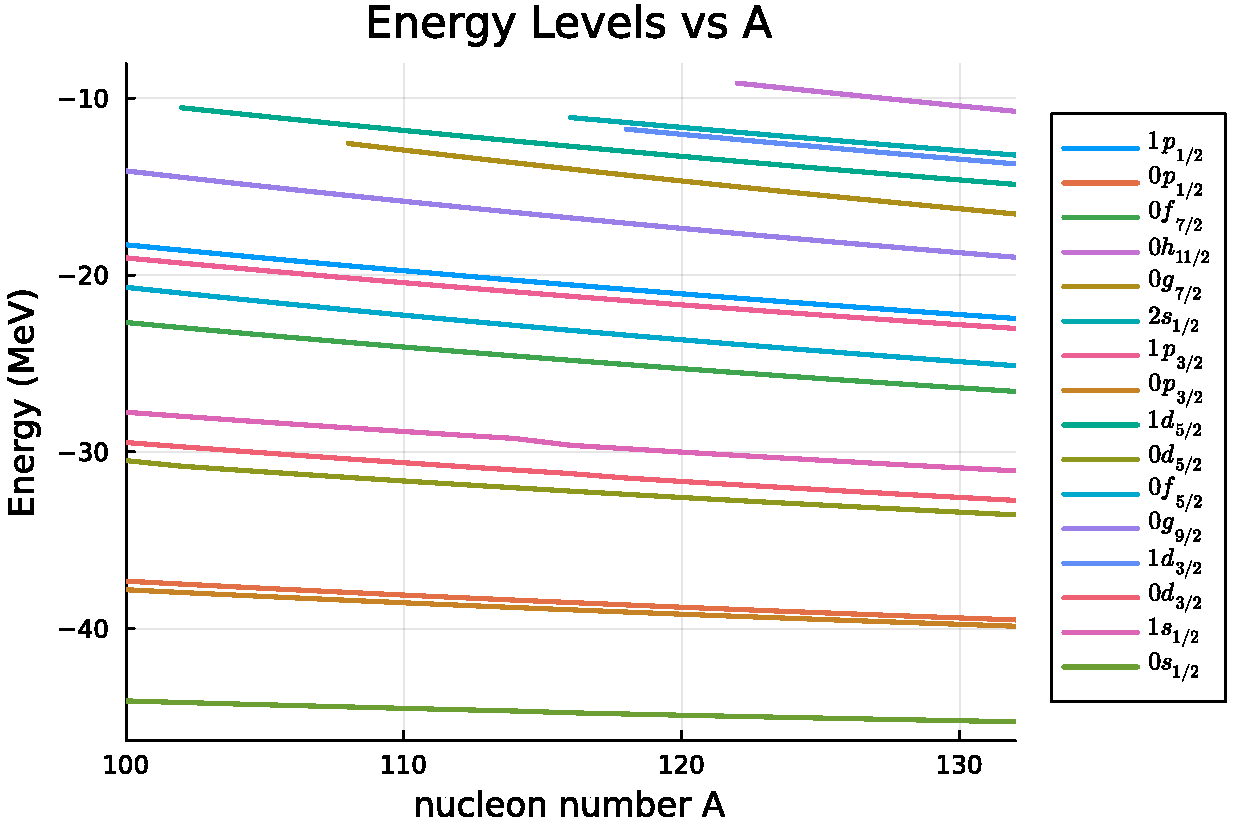
\includegraphics[width=0.8\textwidth]{Energy_vs_A.pdf}
\end{frame}

\begin{frame}{$\Delta$と$g$の質量数依存性}
  \centering
  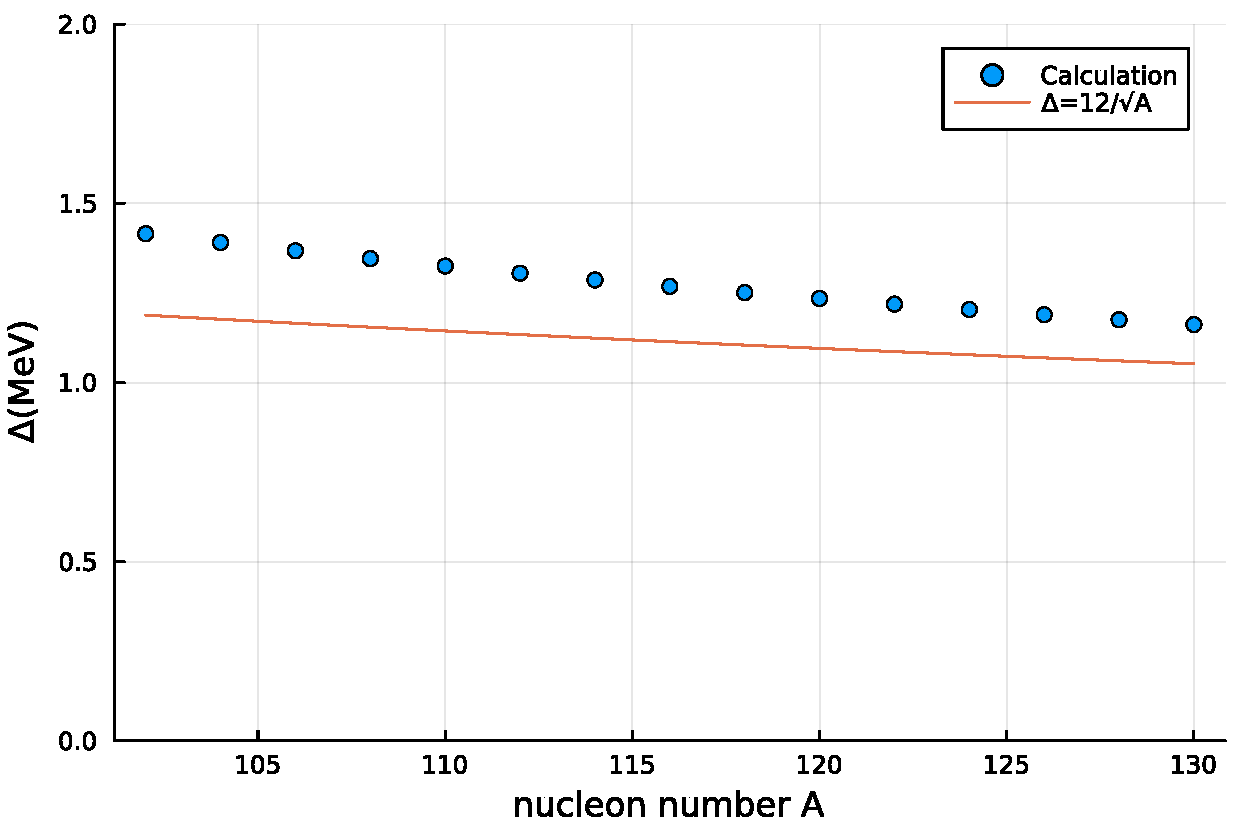
\includegraphics[width=0.6\textwidth]{Delta_vs_A.pdf}\\
  ここで近似式$\Delta=12A^{-1/2}$は文献\cite{nucleus_structure}より。
\end{frame}

\begin{frame}{pairing gapの温度依存性}
  \begin{columns}[totalwidth=1.0\linewidth]
    \begin{column}[t]{0.4\linewidth}
      \begin{itemize}
        \item 全核種で相転移が見られた。
        \item $kT/\Delta_0\sim0.55$付近の傾向が見られる。
        \item $\ce{{}^{102}Sn}$のみ例外的な振る舞い。\\$\Rightarrow$ ペアが1組しか生じないため?
      \end{itemize}
    \end{column}

    \begin{column}[T]{0.6\linewidth}
      \centering
      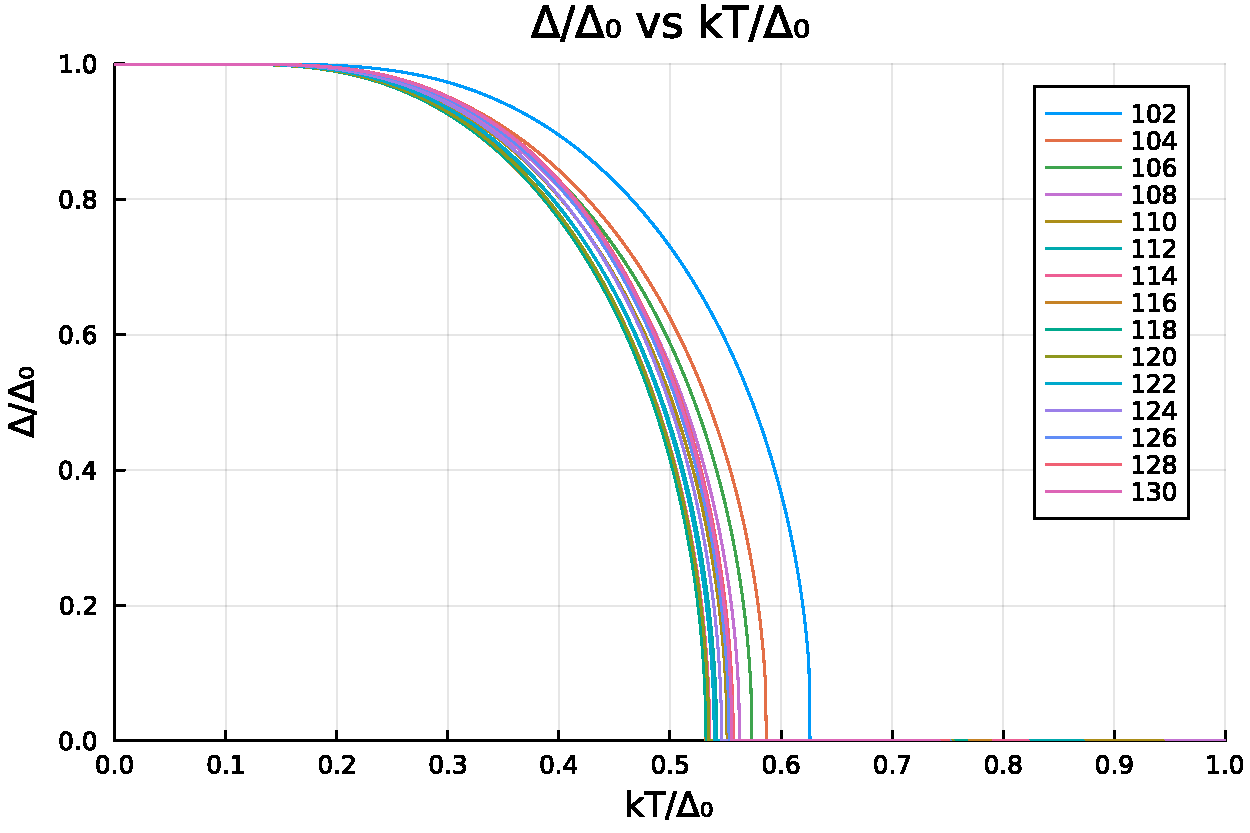
\includegraphics[width=\textwidth]{Comp_FT_dT.pdf}
      \vspace{5pt} % キャプションと画像の間隔調整
      \scriptsize 図1:
  \end{column}
  \end{columns}
\end{frame}

\begin{frame}{エネルギーと比熱の温度依存性}
  \begin{columns}[totalwidth=1.0\linewidth]
    \begin{column}[T]{0.5\linewidth}
      \centering
      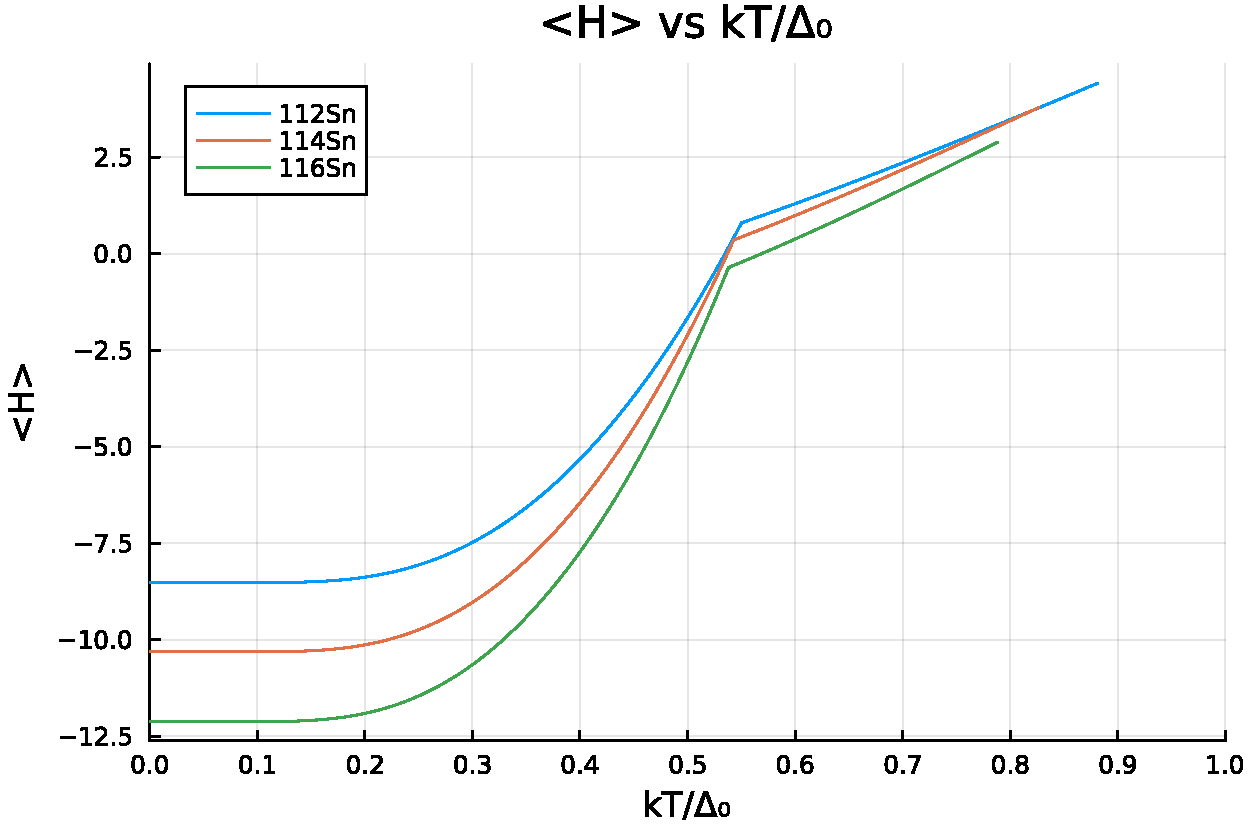
\includegraphics[width=\textwidth]{Comp_FT_H.pdf}
      \vspace{5pt} % キャプションと画像の間隔調整
      \scriptsize 図1:
    \end{column}

  \begin{column}[T]{0.5\linewidth}
    \centering
    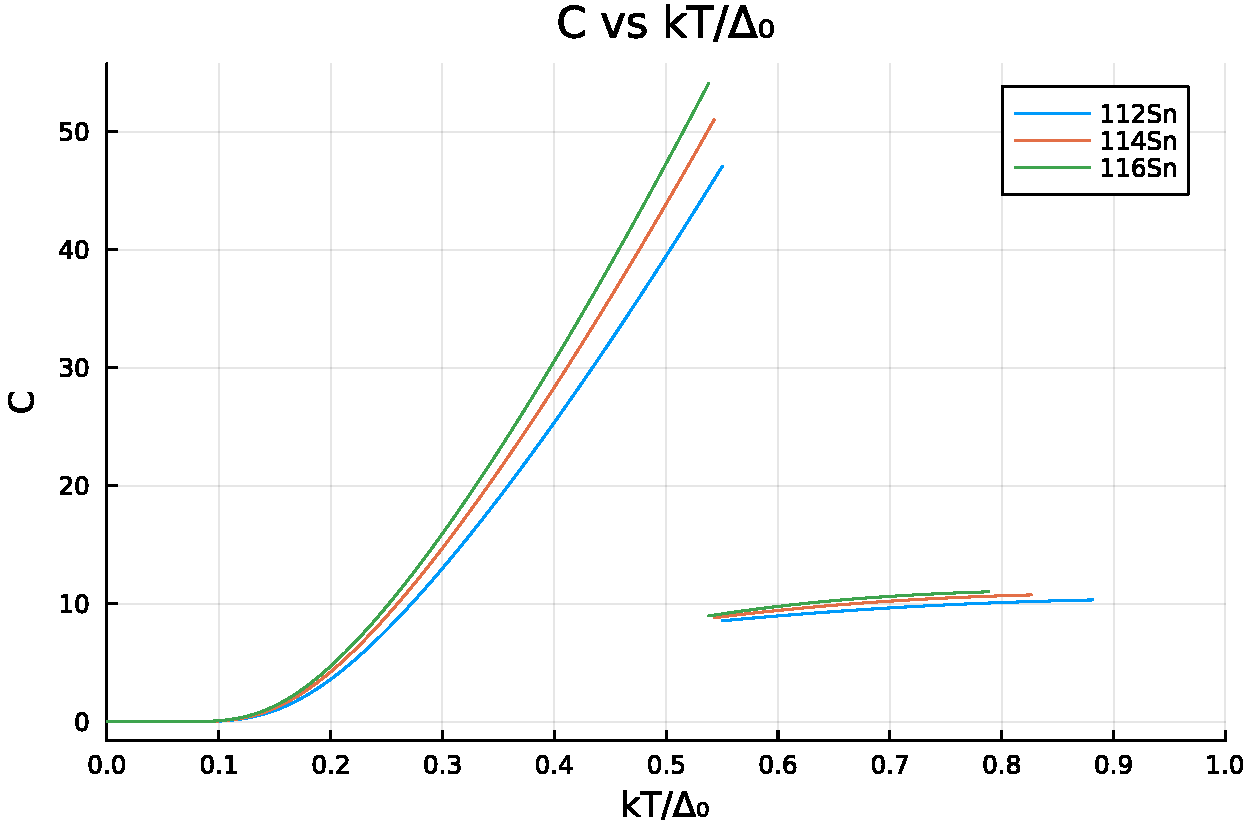
\includegraphics[width=\textwidth]{Comp_FT_C.pdf}
    \vspace{5pt} % キャプションと画像の間隔調整
    \scriptsize 図1:
  \end{column}
  \end{columns}
\end{frame}

\section{結論・課題}

\begin{frame}{結論}
  相転移は高温領域で確認できた。これはエネルギーが上昇することによるpairingの崩壊が原因だと考えられる。
  \par
  比熱においても、相転移温度周辺で急激な変化が見られた。
  
\end{frame}

\begin{frame}{課題}
  今回の解析ではWoods-Saxonポテンシャルとseniority pairingモデルを採用した。
  これらは計算が容易であるが、原子核が球対称であることや、同$j$殻内のpairingのみを考えていることから、
  実際の原子核における波動関数と相互作用を記述する上では、簡単にしすぎている部分も多く存在する。
  これらの課題を解決するためには、変形核にも対応できるような計算を行うのと同時に、相互作用についても
  Gogny相互作用を採用するなど様々な発展が期待できる。\\
  また、今回は一粒子励起のみ考えていたが、集団励起と合わせて考えるとどのような挙動が観測されるのかという
  ことに対しても一定の興味がある。

\end{frame}

\begin{frame}{参考文献}
  \bibliographystyle{jplain}
  \bibliography{list}
\end{frame}

\end{document}
